% ============================================================================
% Resultados do benchmark CGV-Web na máquina modesta (GTX 1050 Ti)
% current (nova) x baseline (antiga). Gerado a partir de
% bench/resultados/gtx1050ti/stats.json (recomputado dos frames brutos em
% bench/dados/gtx1050ti/). Figuras: mesma pasta deste arquivo.
% Compilável isoladamente (pdflatex/tectonic resultados.tex, nesta pasta).
% ============================================================================
\documentclass[11pt,a4paper]{article}
\usepackage[utf8]{inputenc}
\usepackage[T1]{fontenc}
\usepackage[brazil]{babel}
\usepackage{graphicx}
\usepackage{booktabs}
\usepackage[margin=2.5cm]{geometry}
\graphicspath{{./}}

\title{CGV-Web: impacto das otimiza\c{c}\~oes de renderiza\c{c}\~ao em hardware modesto\\ \large Resultados do benchmark automatizado (GTX~1050~Ti)}
\author{}
\date{}

\begin{document}
\maketitle

\section{Metodologia}

Mesma metodologia da m\'aquina de refer\^encia: um \emph{runner} externo ao aplicativo executa
um la\c{c}o \texttt{request\-Animation\-Frame} pr\'oprio e registra o timestamp bruto de cada
quadro apresentado, de forma id\^entica nas duas vers\~oes e sem instrumentar o c\'odigo medido.
Ambas as vers\~oes rodaram na mesma m\'aquina (NVIDIA GTX~1050~Ti, Chrome com limite de FPS
destravado, \emph{viewport} $1920\times1080$, \emph{devicePixelRatio}~1), sobre os mesmos sete
eventos reais do ATLAS (23{,}3~mil a 57{,}4~mil c\'elulas de calor\'imetro), nos tr\^es
cen\'arios usuais: \emph{tour} ($3\times78$~s por evento), \emph{corte parado} e \emph{arraste
do corte} (8~s por eixo). Nesta m\'aquina h\'a uma execu\c{c}\~ao completa por vers\~ao. As
c\'elulas efetivamente renderizadas conferem entre as vers\~oes (diferen\c{c}a de 128 c\'elulas,
at\'e $0{,}65\%$, a favor da vers\~ao antiga).

\section{Resultados}

\begin{table}[htbp]
\centering
\caption{FPS mediano, estabilidade (1\%~low) e \emph{draw calls} por quadro apresentado na
GTX~1050~Ti. ``b'' = baseline (antiga), ``c'' = current (nova).}
\label{tab:gtx}
\small
\begin{tabular}{llrrrrr}
\toprule
Cen\'ario & Evento & C\'elulas & FPS b$\to$c & Speedup & 1\%low b$\to$c & Draws b$\to$c \\
\midrule
tour & 517743$\cdot$363 & 23\,349 & 4{,}2 $\to$ 170 & 40{,}4$\times$ & 3{,}8 $\to$ 131 & 97\,111 $\to$ 49 \\
tour & 518084$\cdot$443 & 23\,612 & 4{,}1 $\to$ 167 & 40{,}5$\times$ & 3{,}7 $\to$ 135 & 98\,063 $\to$ 67 \\
tour & 518084$\cdot$891 & 25\,825 & 4{,}1 $\to$ 164 & 40{,}0$\times$ & 3{,}7 $\to$ 125 & 98\,735 $\to$ 72 \\
tour & 516761$\cdot$342 & 39\,043 & 4{,}1 $\to$ 152 & 36{,}7$\times$ & 3{,}6 $\to$ 124 & 102\,558 $\to$ 129 \\
tour & 520526$\cdot$948 & 40\,976 & 3{,}8 $\to$ 147 & 38{,}8$\times$ & 3{,}3 $\to$ 122 & 107\,033 $\to$ 211 \\
tour & 520249$\cdot$978 & 43\,367 & 3{,}7 $\to$ 145 & 39{,}3$\times$ & 3{,}3 $\to$ 119 & 106\,928 $\to$ 194 \\
tour & 520534$\cdot$398 & 57\,359 & 3{,}5 $\to$ 149 & 43{,}1$\times$ & 3{,}2 $\to$ 124 & 118\,436 $\to$ 214 \\
corte parado & 520534$\cdot$398 & 57\,359 & 3{,}4 $\to$ 147 & 43{,}4$\times$ & 3{,}1 $\to$ 69 & 118\,472 $\to$ 218 \\
arraste $\theta$ & 520534$\cdot$398 & 57\,359 & 4{,}0 $\to$ 127 & 31{,}9$\times$ & 2{,}8 $\to$ 72 & 17\,111 $\to$ 230 \\
arraste $z$ & 520534$\cdot$398 & 57\,359 & 3{,}8 $\to$ 127 & 33{,}8$\times$ & 2{,}0 $\to$ 73 & 17\,722 $\to$ 223 \\
arraste raio & 520534$\cdot$398 & 57\,359 & 4{,}6 $\to$ 125 & 27{,}2$\times$ & 3{,}2 $\to$ 72 & 17\,574 $\to$ 230 \\
\midrule
\multicolumn{4}{l}{M\'edia geom\'etrica dos \emph{speedups} (11 cen\'arios)} & 37{,}4$\times$ & & \\
\bottomrule
\end{tabular}
\end{table}

\paragraph{Vis\~ao geral.}
Na m\'aquina modesta a vers\~ao antiga \'e inutiliz\'avel em todos os cen\'arios: 3{,}4 a
4{,}6~FPS medianos, um quadro a cada ${\sim}0{,}25$~s, muito abaixo do m\'inimo aceit\'avel de
30~FPS. A vers\~ao nova leva os mesmos eventos a 125--170~FPS, acima at\'e do limiar de fluidez
de 60~FPS. O ganho t\'ipico (m\'edia geom\'etrica dos 11 cen\'arios) \'e de
\textbf{37{,}4$\times$} (Tabela~\ref{tab:gtx}, Figura~\ref{fig:speedup-gtx}): 39{,}8$\times$ nos
\emph{tours}, 43{,}4$\times$ no corte parado e 30{,}9$\times$ no arraste do corte. Diferente da
m\'aquina de refer\^encia (RTX~4070~Ti), em que os \emph{tours} ganhavam 7{,}3$\times$, aqui a
CPU domina o custo do quadro em todos os cen\'arios, e o ganho \'e da mesma ordem em todos eles.

\paragraph{Mecanismo.}
A antiga emite 97~mil a 118~mil \emph{draw calls} por quadro apresentado
(Figura~\ref{fig:mecanismo-gtx}); a nova, entre 49 e 230. H\'a nesta m\'aquina um agravante,
medido nos pr\'oprios contadores: no \emph{tour}, a antiga submete ${\sim}7$ renderiza\c{c}\~oes
por quadro que efetivamente chega \`a tela (${\sim}24$ renderiza\c{c}\~oes/s emitidas para
3{,}5 quadros/s apresentados no evento mais pesado) --- trabalho de CPU e GPU descartado, que
n\~ao vira imagem. Por renderiza\c{c}\~ao, o custo \'e o mesmo da m\'aquina forte
(${\sim}17$~mil \emph{draw calls}, vis\'ivel nos arrastes, em que a submiss\~ao \'e 1:1). A
vers\~ao nova, al\'em de reduzir as ordens por quadro em duas ordens de grandeza, submete um
render por quadro apresentado.

\paragraph{Lat\^encia e cauda.}
O \emph{frame-time} t\'ipico da antiga fica em 218--295~ms (o quadro \emph{mediano} j\'a \'e
uma trava percept\'ivel); o p99 chega a 505~ms no arraste em $z$. A nova produz o quadro
t\'ipico em 5{,}9--8{,}0~ms e mant\'em o p99 em 7{,}4--14{,}5~ms --- abaixo do limiar de 60~FPS
at\'e na cauda. No corte parado e nos arrastes o 1\%~low da nova fica em 69--73~FPS, refletindo
os picos peri\'odicos do corte reaplicado; ainda assim, o pior 1\% da nova \'e
${\sim}20\times$ mais r\'apido que a \emph{mediana} da antiga. O eixo azimutal $\varphi$,
in\'edito na vers\~ao nova, mant\'em 127~FPS medianos (1\%~low de 73~FPS; p99 de 14~ms). Abrir
um evento (an\'alise do JiveXML) tamb\'em melhora: de 4{,}9$\times$ a 11{,}8$\times$ mais
r\'apido (t\'ipico 8{,}6$\times$); o pior caso cai de 15{,}0~s para 1{,}3~s.

\paragraph{Amea\c{c}as \`a validade.}
(i)~Uma execu\c{c}\~ao completa por vers\~ao nesta m\'aquina; na m\'aquina de refer\^encia a
varia\c{c}\~ao do \emph{current} entre execu\c{c}\~oes chegou a $36\%$, e essa incerteza de
sess\~ao se aplica aos valores pontuais daqui (a conclus\~ao, com ganho de ordem de grandeza,
n\~ao depende dela). (ii)~No arraste, o \^angulo de abertura registrado difere (180$^\circ$ na
antiga, 110{,}2$^\circ$ na nova), efeito de segunda ordem frente ao ganho medido.
(iii)~C\'elulas renderizadas id\^enticas a menos de 128 unidades; GPU, navegador e
resolu\c{c}\~ao id\^enticos nos metadados. (iv)~Os \emph{draw calls} da antiga s\~ao por quadro
apresentado e embutem o fator de ${\sim}7$ submiss\~oes; por renderiza\c{c}\~ao, a raz\~ao
antiga/nova \'e de ${\sim}75$--$350\times$, como na m\'aquina de refer\^encia.

\begin{figure}[htbp]
  \centering
  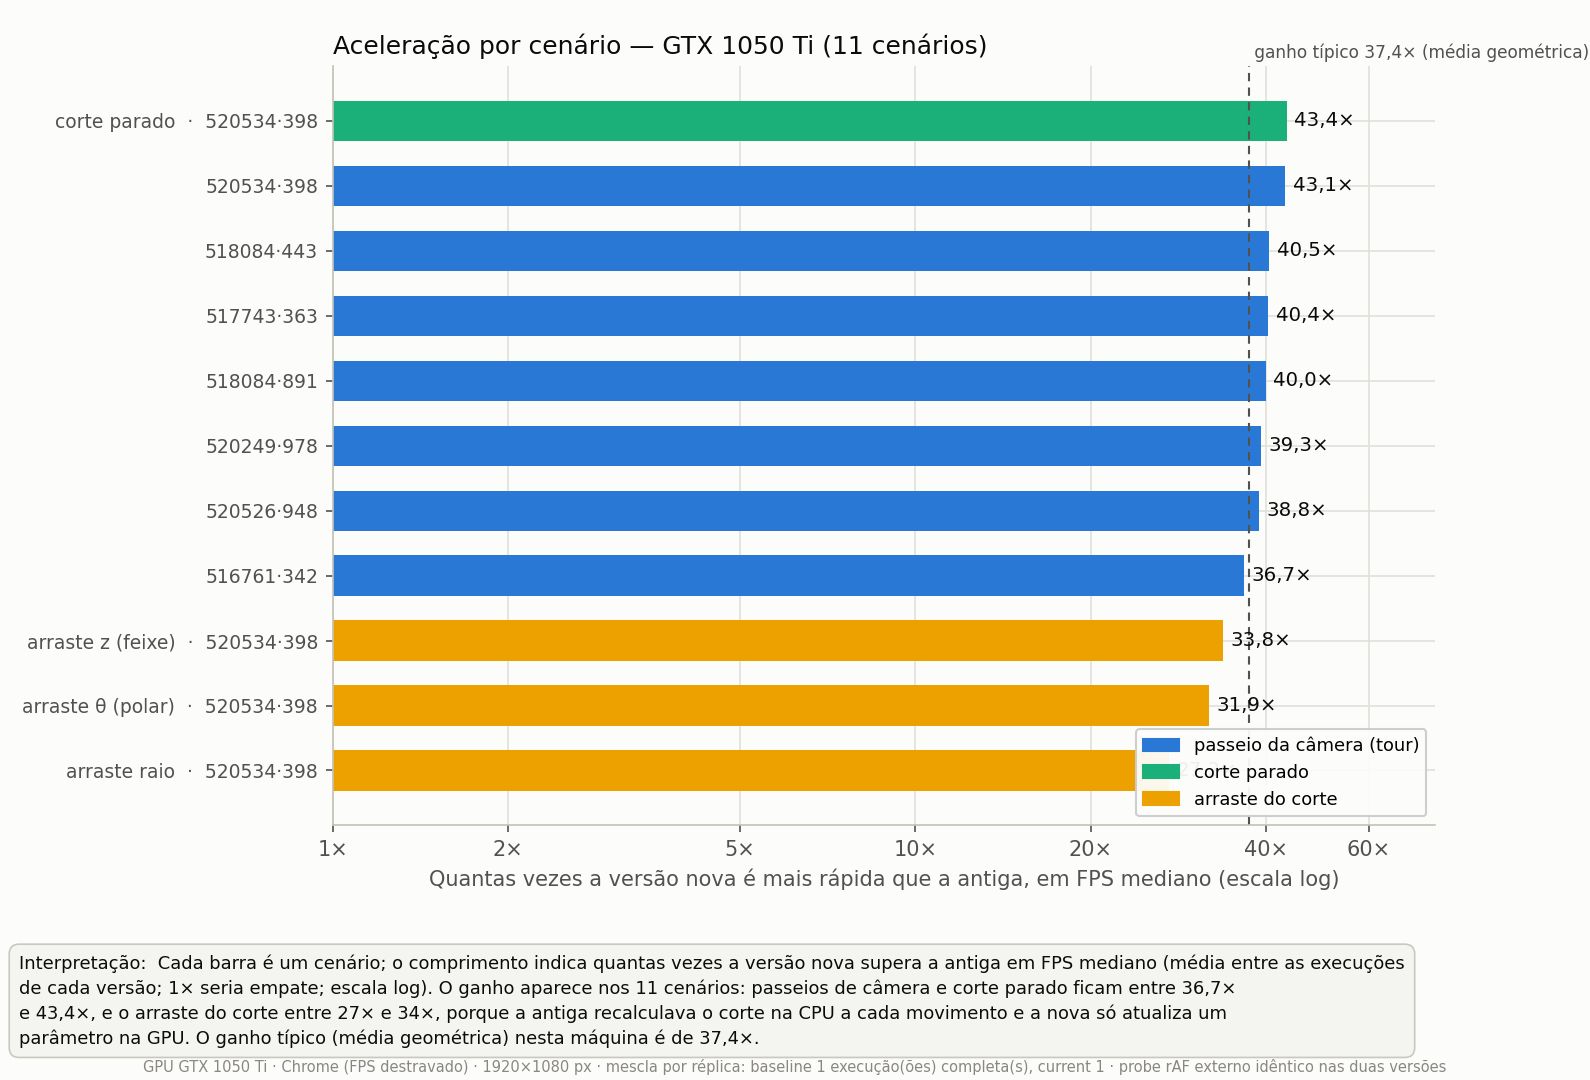
\includegraphics[width=\linewidth]{01_speedup.png}
  \caption{\emph{Speedup} do FPS mediano por cen\'ario na GTX~1050~Ti (escala log). Ganho
  t\'ipico de 37{,}4$\times$; a vers\~ao antiga n\~ao passa de 4{,}6~FPS em nenhum cen\'ario.}
  \label{fig:speedup-gtx}
\end{figure}

\begin{figure}[htbp]
  \centering
  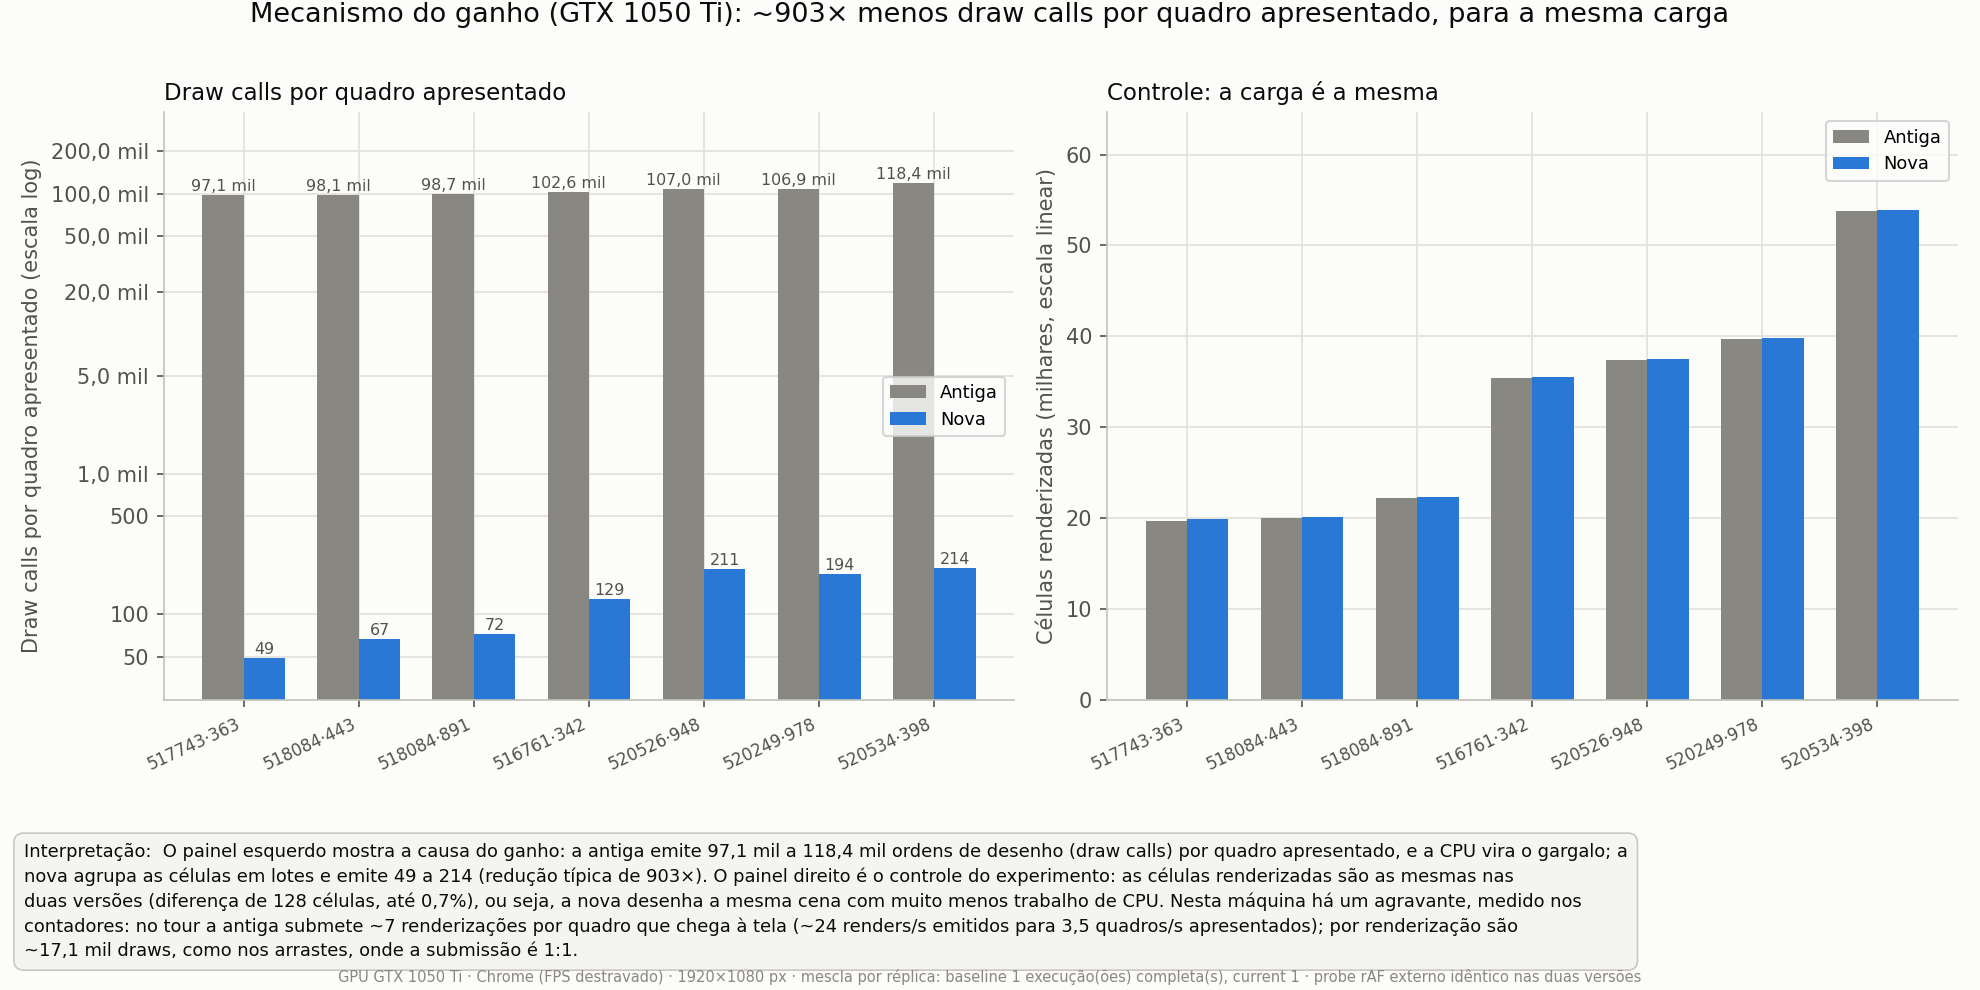
\includegraphics[width=\linewidth]{04_mecanismo.png}
  \caption{Mecanismo na m\'aquina modesta: at\'e 118~mil \emph{draw calls} por quadro
  apresentado (incluindo ${\sim}7$ submiss\~oes de render por quadro que chega \`a tela) contra
  49--230 na vers\~ao nova, para a mesma carga de c\'elulas.}
  \label{fig:mecanismo-gtx}
\end{figure}

\begin{figure}[htbp]
  \centering
  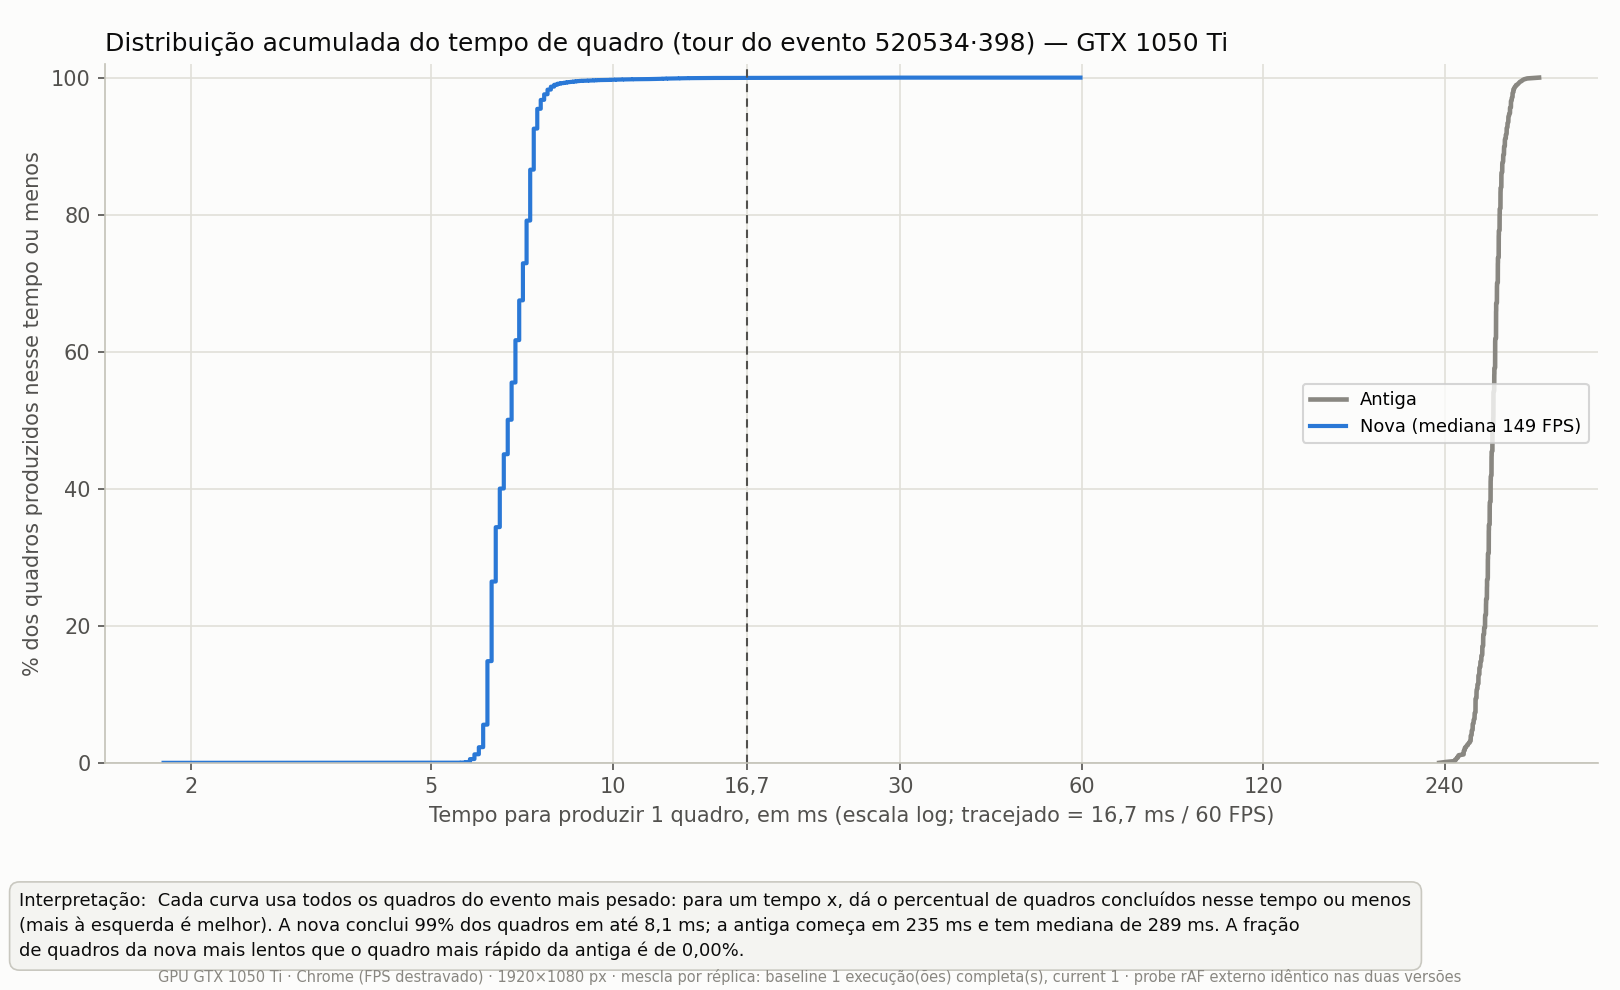
\includegraphics[width=0.85\linewidth]{07_frametime_cdf.png}
  \caption{Distribui\c{c}\~ao acumulada do tempo de quadro no evento mais pesado: a antiga
  inteira acima de 200~ms; a nova inteira abaixo de 16{,}7~ms.}
  \label{fig:cdf-gtx}
\end{figure}

\begin{figure}[htbp]
  \centering
  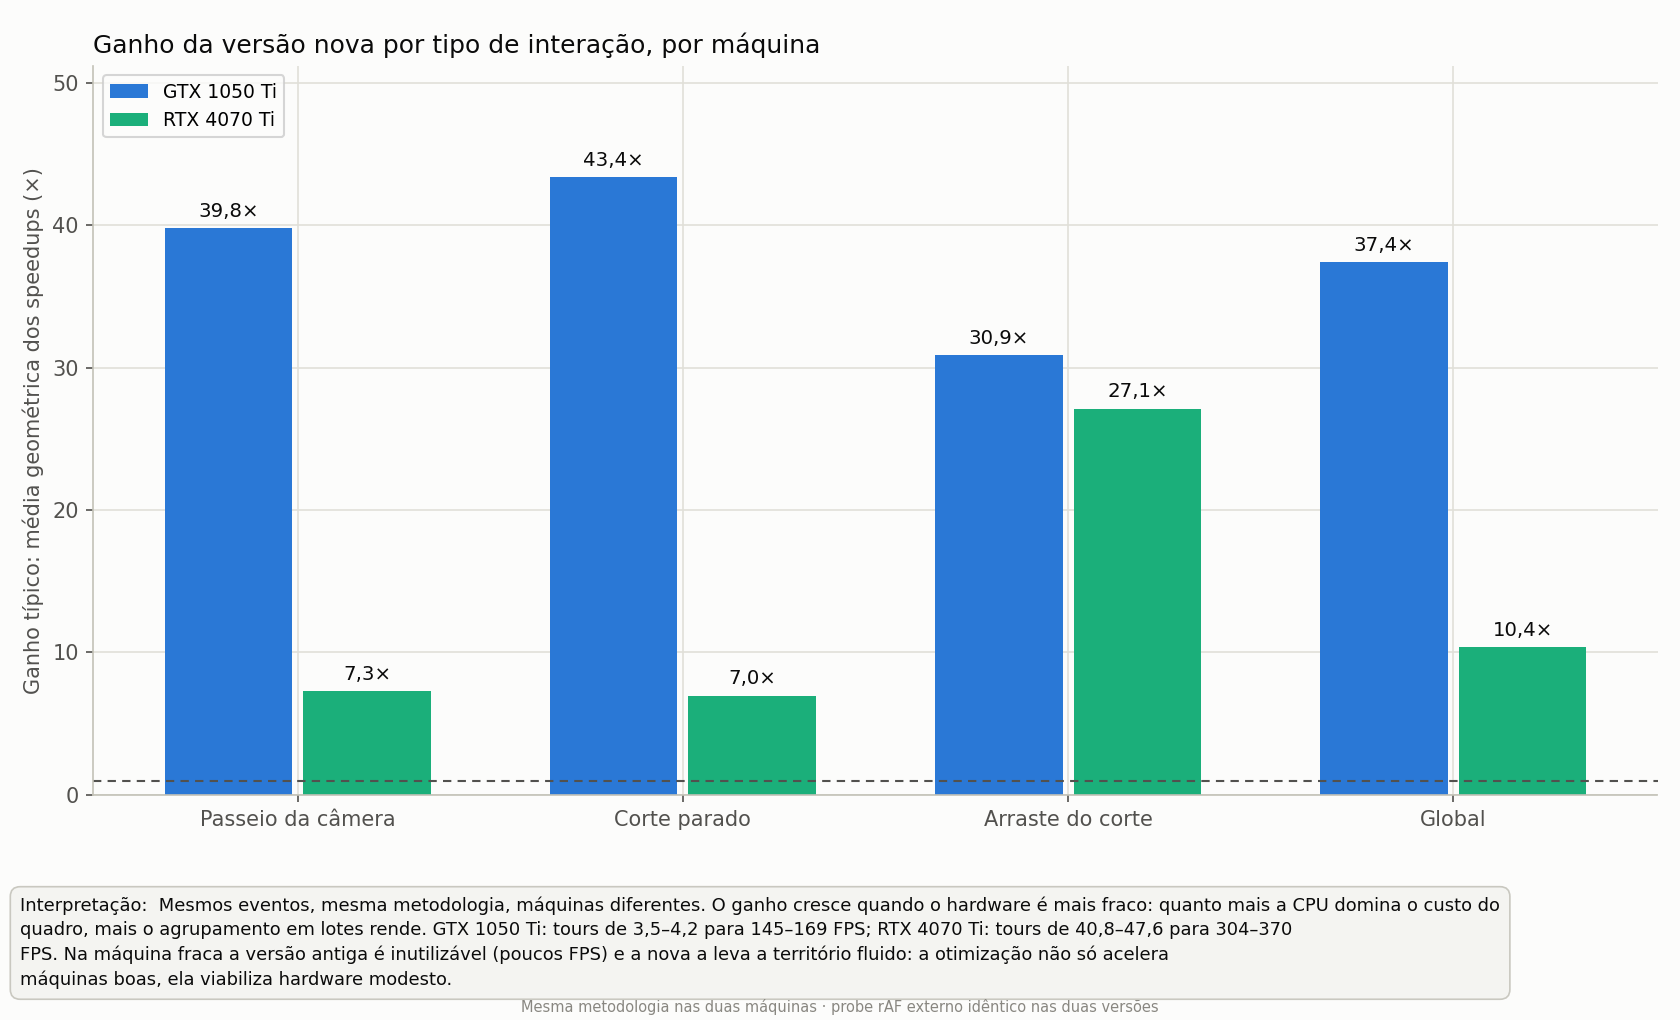
\includegraphics[width=0.9\linewidth]{../comparacao/comparacao_maquinas.png}
  \caption{Ganho por tipo de intera\c{c}\~ao nas duas m\'aquinas: quanto mais fraco o hardware,
  maior o ganho --- a otimiza\c{c}\~ao viabiliza hardware modesto.}
  \label{fig:comparacao}
\end{figure}

\section{Conclus\~ao}

Na m\'aquina modesta o efeito das otimiza\c{c}\~oes \'e qualitativo, n\~ao apenas quantitativo:
a vers\~ao antiga n\~ao \'e utiliz\'avel (3--5~FPS em qualquer cen\'ario), enquanto a nova
sustenta 125--170~FPS nos mesmos eventos --- ganho t\'ipico de 37{,}4$\times$, contra
10{,}4$\times$ na m\'aquina de refer\^encia. O padr\~ao entre m\'aquinas confirma o diagn\'ostico
de gargalo de CPU por \emph{draw calls}: quanto mais fraco o hardware, maior o retorno do
agrupamento em lotes. Para o usu\'ario final, a consequ\^encia pr\'atica \'e que o CGV-Web novo
roda com fluidez em computadores em que a vers\~ao anterior era inoper\'avel.

\end{document}
